\documentclass[a4paper,12pt]{article}

% Se vuoi che il pdf sia in formato mobile, decommenta la linea qui sotto e commenta la prima linea del codice
%\documentclass[1pt]{article}
\usepackage{enumitem}
\usepackage[paper size={90mm, 160mm},left=2mm,right=2mm,top=2mm,bottom=2mm,nohead]{geometry}
\usepackage{microtype}
\setlist[itemize]{leftmargin=*}


\usepackage{float}
\usepackage{url}
\usepackage{xcolor}
\usepackage{pdfpages}
\usepackage{graphicx}


%Comando per creare nuove definizioni stile blocco
\newcommand{\definition}[2]{
	\begin{table}[H]
	\centering
		\begin{tabular}{|p{0.9\linewidth}}
		\textbf{#1}\\ %Titolo della definzione
		#2\\%Testo della definizione
		\end{tabular}
	\end{table}
	\noindent
}

\newcommand{\df}[2]{\definition{#1}{#2}}

%%%%%%%%%%%%%%%%%%%%%%%%%%%%%%%%%%%%%%%%%%%%%%%%%%%%%%%%%%%%%%%%%%%%%
%      INSBOX --- macros for inserting pictures into paragraphs     %
%       Micha\l{} Gulczy\'nski, Szczecin, Jan 1996 / Feb 1998       %
%                     mgulcz@we.tuniv.szczecin.pl                   %
%%%%%%%%%%%%%%%%%%%%%%%%%%%%%%%%%%%%%%%%%%%%%%%%%%%%%%%%%%%%%%%%%%%%%
%
%  version 2.2
%
%  available macros:
%    * \InsertBoxC{anybox}
%        insert a centered box (use int _inside_ a paragraph)
%    * \InsertBoxL{after_line}{anybox}[correction]
%    * \InsertBoxR{after_line}{anybox}[correction]
%        insert a box in the left/right after specified number of lines;
%        correction specified in square brackets is optional;
%        both macros should be called _before_ a paragraph
%    * \MoveBelowBox
%        start a new paragraph just below the current frame
%
%  see the demo.tex file for more information
%

\catcode`\@ = 11
%
%  Margin between the text and the box:
\newdimen\@InsertBoxMargin
\@InsertBoxMargin = 2mm
%
%  definition of \ParShape, an inproved version of plain \parshape
%
\newcount\@numlines    % sum: m_1+...+m_n
\newcount\@linesleft   % counter used when reading lines of \ParShape
\def\ParShape{%
    \@numlines = 0
    \def\@parshapedata{ }% here we'll collect data for plain \parshape
    \afterassignment\@beginParShape
    \@linesleft
}%
\def\@beginParShape{%
    \ifnum \@linesleft = 0
      \let\@whatnext = \@endParShape
    \else
      \let\@whatnext = \@readnextline
    \fi
    \@whatnext
}%
\def\@endParShape{%
    \global\parshape = \@numlines \@parshapedata
}%
\def\@readnextline#1 #2 #3 {% #1 #2 #3 are: m_i, leftskip_i, rightskip_i
    \ifnum #1 > 0
      \bgroup  % I want to keep changes of \dimen0 and \count0 local
        \dimen0 = \hsize
        \advance \dimen0 by -#2  % \parshape requires left skip and
        \advance \dimen0 by -#3  % _length_of_line_ (not right skip!)
        \count0 = 0
        \loop
          \global\edef\@parshapedata{%
            \@parshapedata    % add to \@parshapedata:
            #2                % left skip
            \space            % a space
            \the\dimen0       % length of line
            \space            % another space
          }%
          \advance \count0 by 1
          \ifnum \count0 < #1
        \repeat
      \egroup
      \advance \@numlines by #1
    \fi
    \advance \@linesleft by -1
    \@beginParShape
}%
%
%  \InsertBoxC, \InsertBoxL, \InsertBoxR
%
\newbox\@boxcontent     % box containing the picture to be inserted
\newcount\@numnormal    % number of leading lines to typeset normally
\newdimen\@framewidth   % width of the frame
\newdimen\@wherebottom  % position of frame's bottom
\newif\if@byframe       % true if we are just beside the frame
\@byframefalse
%
%
\def\InsertBoxC#1{%
  \leavevmode
  \vadjust{
    \vskip \@InsertBoxMargin
    \hbox to \hsize{\hss#1\hss}
    \vskip \@InsertBoxMargin
  }%
}%
\def\InsertBoxL#1#2{%
  \@numnormal = #1
  \setbox\@boxcontent = \hbox{#2}%
  \let\@side = 0
  \futurelet \@optionalparameter \@InsertBox
}
\def\InsertBoxR#1#2{%
  \@numnormal = #1
  \setbox\@boxcontent = \hbox{#2}%
  \let\@side = 1
  \futurelet \@optionalparameter \@InsertBox
}%
\def\@InsertBox{%
  \ifx \@optionalparameter [
    \let\@whatnext = \@@InsertBoxCorrection
  \else
    \let\@whatnext = \@@InsertBoxNoCorrection
  \fi
  \@whatnext
}%
\def\@@InsertBoxCorrection[#1]{%
  \ifx \@side 0
    \@@InsertBox{#1}{0}{{\the\@framewidth} 0cm}%
  \else
    \@@InsertBox{#1}{1}{0cm {\the\@framewidth}}%
  \fi
}%
\def\@@InsertBoxNoCorrection{%
  \@@InsertBoxCorrection[0]%
}%
\def\@@InsertBox#1#2#3{%
  \MoveBelowBox
  \@byframetrue
  % \@wherebottom = \pagetotal + (\@numnormal * \baselineskip) +
  %                 (height of \@boxcontent) + (2 * \@InsertBoxMargin)
  \@wherebottom = \baselineskip
  \multiply \@wherebottom by \@numnormal
  \advance \@wherebottom by 2\@InsertBoxMargin
  \advance \@wherebottom by \ht\@boxcontent
  \advance \@wherebottom by \pagetotal
  % I have no idea why, but \InsertBox called at the top of a page
  % calculates space for the box one line too big
  \ifdim \pagetotal = 0cm
    \advance \@wherebottom by -\baselineskip  % ^ reduction
  \fi
  % add the correction
  \advance \@wherebottom by #1\baselineskip
  % \@framewidth = (width of \@boxcontent} + \@InsertboxMargin
  \@framewidth = \wd\@boxcontent
  \advance \@framewidth by \@InsertBoxMargin
  %
  \bgroup  % to keep changes of \dimen0 local
    % check if the box fits in the page
    \ifdim \pagetotal = 0cm
      \dimen0 = \vsize
    \else
      \dimen0 = \pagegoal
    \fi
    \ifdim \@wherebottom > \dimen0
      % print a warning message ...
      \immediate\write16{+--------------------------------------------------------------+}%
      \immediate\write16{| The box will not fit in the page. Please, re-edit your text. |}%
      \immediate\write16{+--------------------------------------------------------------+}%
      % ... and mark this place in document with a black box
      \vrule width \overfullrule
    \fi
  \egroup
  \prevgraf = 0
  % insert the box in the left (if #2 = 0) or in the right (if #2 = 1)
  \vbox to 0cm{%
    \dimen0 = \baselineskip
    \multiply \dimen0 by \@numnormal
    \advance \dimen0 by -\baselineskip
    \setbox0 = \hbox{y}%
    \vskip \dp0
    \vskip \dimen0
    \vskip \@InsertBoxMargin
    \ifnum #2 = 1
      \vtop{\noindent \hbox to \hsize{\hss \box\@boxcontent}}%
    \else
      \vtop{\noindent \box\@boxcontent}%
    \fi
    \vss
  }%
  % I have no idea why, but this is really necessary
  \vglue -\parskip
  \vskip -\baselineskip
  % each following paragraph needs to be formatted properly
  \everypar = {%
    % are we already below the bottom of the box?
    \ifdim \pagetotal < \@wherebottom
      % no...
      \bgroup  % to keep some changes local
        % let's calculate parameters for \ParShape
        \dimen0 = \@wherebottom
        \advance \dimen0 by -\pagetotal
        \divide \dimen0 by \baselineskip
        \count1 = \dimen0
        \advance \count1 by 1
        \advance \count1 by -\@numnormal
        \ifnum #2 = 1
          \ParShape = 3
                      {\the\@numnormal}   0cm   0cm
                      {\the\count1}       0cm   {\the\@framewidth}
                      1                   0cm   0cm
        \else
          \ParShape = 3
                      {\the\@numnormal}   0cm                  0cm
                      {\the\count1}       {\the\@framewidth}   0cm
                      1                   0cm                  0cm
        \fi
      \egroup
    \else
      % yes!
      \@restore@    % it's time to end everything
    \fi
  }%
  % this definition isn't very necessary --- just in case the paragraph
  % following \InsertBoxL or \InsertBoxR has fewer lines that the
  % first argument of the macro
  \def\par{%
      \endgraf
      \global\advance \@numnormal by -\prevgraf
      \ifnum \@numnormal < 0
        \global\@numnormal = 0
      \fi
      \prevgraf = 0
  }%
}%
%
%  call this macro to move the current position just below the
%  current frame
%
\def\MoveBelowBox{%
  \par
  \if@byframe
    \global\advance \@wherebottom by -\pagetotal
    \ifdim \@wherebottom > 0cm
      \vskip \@wherebottom
    \fi
    \@restore@
  \fi
}%
%
%  normal settings are as follows:
%
\def\@restore@{%
    \global\@wherebottom = 0cm
    \global\@byframefalse
    \global\everypar = {}%
    \global\let \par = \endgraf
    \global\parshape = 1 0cm \hsize
}%
%
%  someone told me that in LaTeX there is no \pageno counter;
%  the counterpart is \c@page
%
\ifx \documentclass \@Dont@Know@What@It@Is@
\else
  \let \pageno = \c@page
\fi


\catcode`\@ = 12

\newcommand{\lessonDate}[1]{\InsertBoxR{0}{\tiny{#1}}}

\newcommand{\E}{\`E\space}

\usepackage{listings}
\lstset{language=C++,
                keywordstyle=\color{blue},
                stringstyle=\color{red},
                commentstyle=\color{green},
                morecomment=[l][\color{magenta}]{\#}
}

\begin{document}

\begin{titlepage}
\begin{center}
	\Large{\textbf{Gestione dell'informazione Geospaziale}}
\vfill
\normalsize{Caccaro Sebastiano}\\
\normalsize{A.A.2019/2020}
\end{center}
\end{titlepage}
\tableofcontents

\clearpage


%Lunedi 7 ottobre
\lessonDate{7 Ottobre 2019}
\section{Introduzione}
\textbf{Geospaziale} tratta di dati sulla superficie terrestre. Posso trattare vari tipi di spazi, anche su unità di misura diverse, come lo spazio-tempo.

\subsection{Aspetti organizzativi}
\subsubsection{Obiettivi}
Concetti base:
\begin{itemize}
	\item Acquisizione dei dati
	\item Gestione dei dati: li mantengo in dei DBMS spaziali.
	\item Analisi dei dati, clustering (= raggruppare oggetti in base a criteri di omogeneità) ecc.
\end{itemize}

\subsubsection{Organizzazione del corso}
Il corso verrà così articolato:
\begin{itemize}
	\item Concetti base
	\item DBMS Spaziali
	\item Rappresentazione di oggetti in movimento
	\item Analisi dei dati spaziali.	
\end{itemize}

\textbf{Bisogna sapere PostgreSQL!}\\
L'esame consiste in un progetto più di un orale (potrebbe diventare una prova scritta all'ultima lezione del corso).\\
Il sito del corso è \url{homes.di.unimi.mdamiani/corsi/gig/}\\
\textbf{User}: gis7 \textbf{Pwd:} sql07sql

\subsubsection{Materiale}
\E presente un libro in formato PDF sul sito della docente.


\subsection{Concetti Base}
\subsubsection{Esempio di OpenStreetMaps}
OpenStreetMaps è una \textbf{mappa} aperta \textbf{collaborativa}, sostanzialmente un disegno. Ma non ci interessano i colori delle strade ecc. Cosa vuol dire Mappa Collaborativa?
\begin{itemize}
 \item \textbf{Mappa} è una banca dati che contiene informazioni geografiche coerenti, che poi vengono rappresentate tramite una mappa.
 \item \textbf{Collaborativa} la base di dati è modificabile da chiunque.\\
\end{itemize}


Costruire mappe è sempre stato altamente dispendioso, sopratutto per quanto riguarda l'acquisizione dei dati. OpenStreetMaps rende facile il reperimento e l'uso di dati spaziali.

\subsubsection{Spazio}
Parliamo di spazio geometrico con longitudine e latitudine, che vogliono una posizione e un sistema di riferimento. \E però molto più facile usare lo spazio cartesiano. Lo spazio simbolico invece rappresenta dei luoghi anche in base alla loro funzione (esempio cartine indoor). A seconda del tipo di spazio che sto analizzando, cambia anche la nozione di distanza. Ad esempio, come misuro la distanza in ambiente indoor?\\
Un oggetto può avere vari tipi di proprietà:
\begin{itemize}
\item \textbf{Geometriche}: forma
\item \textbf{Topografiche}: i collegamenti, a mo di grafo
\item \textbf{Tematiche}: caratteristiche, ad esempio i il numero di abitanti di un edificio
\end{itemize}

Ci possono essere movimenti di tipo:
\begin{itemize}
\item \textbf{Continuo:} ad esempio, movimento di palla nello spazio.
\item \textbf{Discreto:} ho un numero di posizioni finito, ad esempio posso essere in un dato momento solo sotto una cella telefonica.
\end{itemize}

%Possibile spostare a mappe
\E importantissimo poter visualizzare i dati. Altrimenti, non riesco a farmi un'idea di cosa ho in mano.

\subsubsection{Acquisizione dei dati}
Ci sono vari strumenti e metodi (arei, GPS, ecc.).\\
La posizione non è mai precisa al 100\%. I dati geospaziali dovrebbero essere sempre accompagnati anche dalla misura della loro incertezza.

\subsubsection{Trattamento dei dati}
Sono presenti varie tecnologie che permettono di gestire e trattare i dati raccolti:
\begin{itemize}
\item \textbf{Sistemi GIS}: piattaforme software (= programmoni) che mi permettono di:
	\begin{itemize}
		\item Acquisire dati: digitalizzarli, controllarne la correttezza, integrare dati eterogenei (con fonti e caratteristiche diverse).
		\item Archiviare e accedere ai dati
		\item Trattare i dati
		\item Visualizzare dati
	\end{itemize}
\item \textbf{DBMS spaziali}: DBMS normali arricchiti con tipi e operazioni per dati spaziali. Praticamente sono SQL con estensioni spaziali.
	
\item Package specializzati.
\end{itemize}

\lessonDate{11 Ottobre 2019}
\section{Coordinate Geospaziali}
\definition{Geodesia}{Disciplina che studia la forma della Terra, le sue dimensioni, i metodi per determinare la posizione dei punti sulla sua superficie.}

\definition{Cartografia}{Disciplina che ha per oggetto la rappresentazione grafica, in proporzioni ridotte, della superficie terrestre o di una parte di essa, dei suoi aspetti caratteristici, fenomeni che si svolgono e la preparazione e la costruzione delle carte geografiche.}

Le coordinate sono delle tuple di numerici che hanno senso in un sistema di riferimento (CRS - Coordinate Reference System). Bisogna distinguere due tipi di coordinate:
\begin{itemize}
\item \textbf{Coordinate Geografiche:} ex Latitudine e longitudine.
\item \textbf{Coordinate Proiettate:} ovvero proiettate su un piano.
\end{itemize}
\E possibile anche fornire delle coordinate indirette, come un indirizzo postale, IP, ecc. Questi metodi vengono poi mappati a coordinate.

\subsection{Coordinate Geografiche}
\definition{Meridiano}{Semicirconferenza che unisce i due poli.}
\definition{Meridiano di Greenwich}{Anche detto Meridiano Fondamentale". Meridiano di riferimento per il calcolo della circonferenza.}
\definition{Piano Equatoriale}{Piano che ha come proiezione l'equatore.}

\begin{figure}[H]
	\centering
	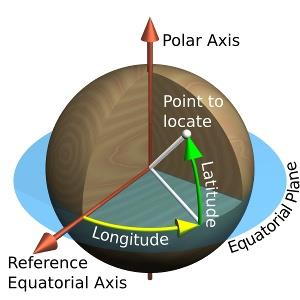
\includegraphics[width=.4\linewidth]{Immagini/LatLong.png}
\end{figure}

\subsection{Latitudine e longitudine}
\df{Longitudine}{Angolo sul piano di meridiano fra l'equatore e la linea passante per P e perpendicolare alla superficie terrestre. Indicata con phi.}\\
\df{Latitudine}{Angolo sul piano equatoriale formato dal piano del meridiano passante per P e il piano del meridiano fondamentale. Indicata con lambda}\\

Sia latitudine e longitudine sono angoli, quindi si misurano in gradi. Ma ci sono 2 modi per esprimerli:
\begin{itemize}
\item \textbf{Sistemi sessasegimali:} Misuro in sessantesimi.
\item \textbf{Sistemi digitali:} Misure in frazioni decimali di grado.
\end{itemize}

La longitudine è espressa fra \textbf{180 OVEST} e \textbf{180 EST} (-180 e 180). La latitudine è espresso fra \textbf{90 NORD} E \textbf{90 SUD} (0 -90 e 90). Per ovvi motivi, nei poli la longitudine non è definita.\\

\subsection{Distanza}
Chiaramente, per calcolare la distanza, non basta tirare una linea. La distanza più breve fra due punti, non è una linea retta sul piano.

\definition{Cerchio Massimo}{Circonferenza che risulta dall'intersezione di un piano passante per il centro e la superficie terrestre. Il cerchio massimo è un esempio di geodetica}
\definition{Distanza di Cerchio Massimo}{Distanza più breve tra 2 punti A e B è data dall'arco di cerchio massimo passante per A e B (con estremi A e B). Ipotesi di Terra sferica (errore stimato 0.3\%)}

\begin{figure}[H]
	\centering
	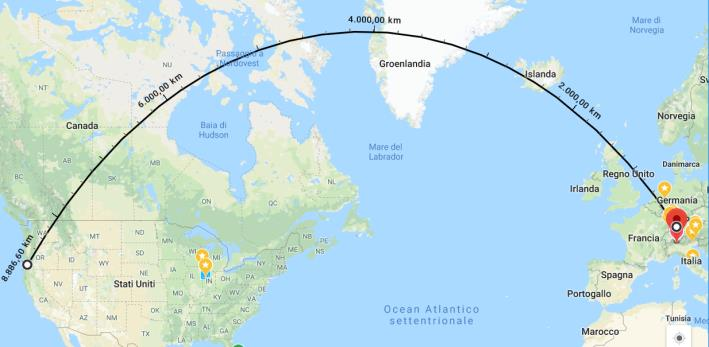
\includegraphics[width=.75\linewidth]{Immagini/CMax.png}
	\caption{Distanza più breve (di cerchio massimo) fra due punti sulla terra}
\end{figure}

\subsection{Forma della Terra}
La terrà non è una sfera, ci sono valli, montagne, ecc. Dobbiamo quindi stabilire una superficie di riferimento, un modello geometrico, \textbf{datum geodetico}. Una prima approssimazione potrebbe essere il geoide, che "taglia" le montagne e pone il livello di riferimento alla superficie del mare.
Sarebbe però troppo difficile da computare, quindi usiamo un modello regolare detto \textbf{Ellissoide}. Sono stati definiti vari tipi di ellissoide. Ciò è causato da vari fattori. Alcuni ellissoidi approssimano meglio alcune aree geografiche (es Europa, Italia ecc) (datum locale), mentre altri cercano di approssimare tutta la superficie terrestre senza fare troppe preferenze. La tendenza è quella di migrare verso dei modelli globali (datum globale), come WGS84, usato nel GPS.\\
Va da sè che latitudine e longitudine non sono sufficienti per identificare univocamente un punto, ma è necessario anche  il codice dell'ellissoide.

\begin{figure}[H]
	\centering
	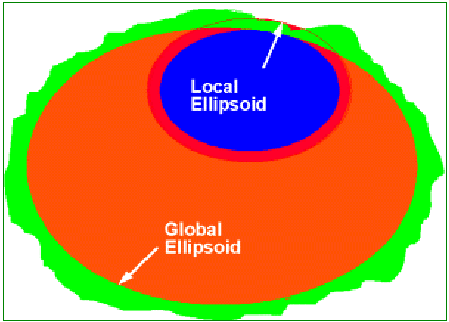
\includegraphics[width=.75\linewidth]{Immagini/Elix.png}
	\caption{Ellissoidi locali e globali}
\end{figure}

\subsubsection{Trasformazione di datum}
Può dover essere necessario eseguire delle trasformazioni di datum fra modelli geodetici differenti.

\subsection{Coordinate Proiettate}
Consistono sostanzialmente in un mapping da coordinate geografiche a coordinate cartesiane. \E possibile passare da una proiezione all'altra senza perdita di dettagli tramite alcune formulette matematiche.\\
Ovviamente, questa mappatura causa delle deformazioni, e in base a queste posso classificare le proiezioni:
\begin{itemize}
\item \textbf{Equivalenti:} mantengono le aree
\item \textbf{Conformi:} mantengono gli angoli
\item \textbf{Equidistanti: } mantengono le distanze
\end{itemize}
Non esistono proiezioni migliori, ma solo più ideali rispetto al contesto.



%\definition{Legge di Brooks}{Aggiungere personale ad un progetto in ritardo lo farà solo ritardare.}

\end{document}